\documentclass[twocolumn,           % Format : preprint, twocolumn
%\documentclass[preprint,           % Format : preprint, twocolumn
               showpacs,            % Pacs : showpacs, noshowpacs
               preprintnumbers,     % Preprint: preprintnumbers,
               			    %           nopreprintnumbers
               aps,                 % Society: ...
               prl,          	    % Journal Style : pra, prb, prc, prd, pre,
               			    %                 prl, prstab, rmp
               letterpaper,             % Size : a4paper, ...
               superscriptaddress,      % Affiliation (Title) : groupedaddress,
                                    %                       superscriptaddress,
                                    %                       unsortedaddress
               nofootinbib,         % Footnote: footinbib, nofootinbib
               tightenlines,        % Remove additional spaces in a line
               floats,floatfix      % Floating pictures and tables
               ,usenatbib,
               ]{revtex4-1}
\usepackage{graphicx}  % needed for figures
\usepackage{dcolumn}   % needed for some tables}
%\usepackage[style=authoryear,backend=biber]{biblatex}
\usepackage{bm}        % for math
\usepackage{amsmath,amssymb}
\usepackage{hyperref}
\usepackage{color}
\definecolor{purple}{rgb}{0.58,0.0,0.83}
\usepackage{caption}
\usepackage[toc,page]{appendix}
\usepackage{subcaption}

\begin{document}

\title{Constraining two field inflationary models}
\author{Luis Padilla-Albores}  
\email{epadilla@fis.cinvestav.mx}
\affiliation{Departamento de F\'isica, Centro de Investigaci\'on y de Estudios Avanzados del IPN, A.P. 14-740, 07000 M\'exico D.F.,
  M\'exico.}
   \author{Jos\'e Alberto V\'azquez Gonz\'alez}  
\email{javazquez@icf.unam.mx}
\affiliation{Instituto de ciencias físicas, Universidad Nacional Aut\'onoma de M\'exico, sede Cuernavaca, Morelos, México}
\author{Tonatiuh Matos}  
\email{tmatos@fis.cinvestav.mx}
\affiliation{Departamento de F\'isica, Centro de Investigaci\'on y de Estudios Avanzados del IPN, A.P. 14-740, 07000 M\'exico D.F.,
  M\'exico.}
\date{\today}

\begin{abstract}
\textcolor{red}{Nota: No tuve mucho cuidado en que lo que llevo tenga una buena estructura ya que no s\'e a\'un si este paper se dividir\'a en 2 o no. Ya que decidamos como ser\'a este paper le dar\'e la estructura correspondiente. Saludos.}

\end{abstract}
\pacs{????}
\begin{keywords}
dark matter  -- galaxy clusters --  gravitation  -- relativity
\end{keywords}

\maketitle



\section{Introduction}
\label{introduction}

XXXXX

XXXXX

XXXXX

XXXXX

XXXXX

\section{Generalities for two field inflationary models}

Although one scalar field models for inflation can be preferable given the fact that they predict only adiabatic like perturbations, two field models can be interesting since there are some regions of parameters were this models can generate small isocurvature perturbations and the addition of new free parameters can help to ''death" single-field inflationary models to bring them back.  

In this section we review in a general way two field inflationary models for inflation following (Ref. Christian T. Byrnes and David Wands). 

\subsection{Background equation of motion}

In this section we consider a two-field inflationary model with canonical kinetic term and where its dynamics is described by an arbitrary interaction potential $V(\phi,\psi)$. As usual we consider that the classical fields are homogeneous and evolve in a FLRW background. Then, the background equation of motion for each scalar field and the Hubble parameter are
\begin{subequations}
\begin{equation}\label{KGEq}
\ddot{\phi}_i+3H\dot{\phi_i}+\frac{dV_i}{d|\phi_i|^2}\phi_i=0 \ \ \ (i=\phi,\psi)
\end{equation}
\begin{equation}
H^2=\frac{8\pi G}{3}\left[V+\frac{1}{2}\left(\dot{\phi}+\dot\psi\right)\right],
\end{equation}
\end{subequations}
where $V_i\equiv\partial V/\partial \phi_i$. In the inflationary era it is usually assumed that the scalar fields are slow-rolling. This happens always that the condition $\epsilon_i,|\eta_{ij}|\ll 1$ is fulfill; $\epsilon_i$ and $\eta_{ij}$ are called the slow-roll parameters and are defined in appendix [A]. If this happens we can rewrite the above equations as
\begin{subequations}
\begin{equation}
\dot{\phi}_i\simeq \frac{2}{3}\epsilon_i V
\end{equation}
\begin{equation}
H^2\simeq \frac{8\pi G}{3}V\left(1+\frac{1}{3}\epsilon^H\right)
\end{equation}
\end{subequations}
where $\epsilon^H$ are new slow-roll parameters defined in appendix [A]. 
\subsection{The adiabatic and isocurvature perturbations}

The equation of motion for the perturbed fields in the spatially flat gauge are (ref)
\begin{equation}
\ddot{\delta\phi}_i+3H\dot{\delta\phi}_i+\sum_j\left[V_{ij}-\frac{8\pi G}{a^3}\frac{d}{dt}\left(\frac{a^3}{H}\dot{\phi}_i \dot\phi_j\right)\right]\delta\phi_j=0
\end{equation}
For the large scales ($k\ll aH$) it is better to work in a rotating basis of the fields given by
  \begin{subequations}
  \begin{equation}
  \binom{\delta \sigma}{\delta s}=S^{\dagger}\binom{\delta \phi}{\delta\psi}
  \end{equation}
  where
  \begin{equation}\label{angle}
  S=\begin{pmatrix}\cos\theta & -\sin\theta\\ \sin\theta & \cos\theta\end{pmatrix}, \ \ \ \tan\theta =\frac{\dot \psi}{\dot \phi}\simeq\pm \sqrt{\frac{\epsilon_\psi}{\epsilon_\phi}}
  \end{equation} 
  \end{subequations}
The field $\sigma$ is parallel to the trajectory and is usually called \textit{adiabatic field} while the field  $s$ is perpendicular to it and is called \textit{entropy field}. 

 If the background trajectory is curved it happens that $\delta\sigma$ and $\delta s$ are correlated at Hubble exit. In this way the power spectrum and cross-correlation at Hubble exit is given by
\begin{subequations}
\begin{equation}
P_{\sigma^*}((k))\simeq\left(\frac{H_*}{2\pi}\right)^2(1+(-2+6C)\epsilon-2C\eta_{\sigma\sigma})
\end{equation}
\begin{equation}
C_{\sigma s^*}(k)\simeq-2C\eta_{\sigma s}\left(\frac{H_*}{2\pi}\right)^2
\end{equation}
\begin{equation}\label{5c}
P_{s^*}(k)\simeq\left(\frac{H_*}{2\pi}\right)^2(1+(-2+2C)\epsilon-2C\eta_{ss})
\end{equation}
\end{subequations}
where $C\simeq 0.7296$ and $\epsilon$ and $\eta_{ij}$ ($i,j=\sigma,s$) are new slow-roll parameters defined in term of the new adiabatic and entropy fields (see appendix [A]).
\subsection{Final power spectrum and spectral index}
The curvature and isocurvature perturbations are defined as
\begin{equation}\label{RS}
R\equiv\frac{H}{\dot\sigma}\delta \sigma, \ \ \ S=\frac{H}{\dot \sigma}\delta s
\end{equation}
In the slow-roll limit in large scales, the evolution of curvature and isocurvature perturbations can be written using the formalism of tranfer matrix (ref) as
\begin{equation}
\binom{R }{S}=\begin{pmatrix}1 & T_{RS}\\ 0& T_{SS}\end{pmatrix}\binom{R}{S}_*
\end{equation}
where
\begin{subequations}
\begin{equation}
T_{SS}(t^*,t)=\exp\left(\int^t_{t^*}\beta Hdt'\right), \ \ \
\end{equation}
\begin{equation}\label{TRS}
T_{RS}(t^*,t)=\exp\left(\int^t_{t^*}\alpha T_{SS}Hdt'\right)
\end{equation}
\end{subequations}
and at linear order in slow-roll parameters
\begin{equation}
\alpha\simeq -2\eta_{\sigma s}, \ \ \ \ \beta\simeq-2\epsilon+\eta_{\sigma\sigma}-\eta_{ss}
\end{equation}

In the other side the primordial curvature perturbation, during radiaton-dominates era some time after inflation has ended, is given in large scales by
\begin{equation}
R=\Psi+\frac{H\delta\rho}{\rho}
\end{equation}
where $\Psi$ is the gravitational potential. The conventional definition of the isocurvature perturbation for an $i$ specie is given relative to the radiation density by
\begin{equation}
S_i=H\left(\frac{\delta\rho_{i}}{\rho_{i}}-\frac{\delta\rho_\gamma}{\rho_\gamma}\right).
\end{equation}
Then, the final power spectrum at the beginning of the radiation-domination era is given by
\begin{subequations}\label{spectrums}
\begin{equation}\label{PRf}
P_R\simeq P|_*(1+\cot^2\Delta),
\end{equation}
\begin{equation}
P_S=T^2_{SS}P|_*,
\end{equation}
\begin{equation}
C_{RS}=T_{RS}T_{SS}P_R|_*
\end{equation}
\end{subequations}
where at linear order in slow-roll parameters
\begin{equation}
P|_*=\frac{1}{2\epsilon}\left(\frac{H_*}{2\pi M_{pl}}\right)^2
\end{equation}
with $M_{pl}$ the Planck mass and $\Delta$ is the observable correlation angle defined at lower order as
\begin{equation}
\cos\Delta =\frac{T_{RS}}{\sqrt{1+T_{RS}^2}}.
\end{equation}
The final scalar tilts, defined as $n_x-1=d\ln P_x/d\ln k$, at linear order in slow-roll parameters are
\begin{subequations}\label{tilts}
\begin{eqnarray}
n_R-1&\simeq & -(6-4\cos^2\Delta)\epsilon+2\sin^2\Delta\eta_{\sigma\sigma}\nonumber \\ &&+4\sin\Delta\cos\Delta\eta_{\sigma s}+2\cos^2\Delta\eta_{ss}\\
n_c-1&\simeq &-2\epsilon+2\tan\Delta\eta_{\sigma s}+2\eta_{ss}\\
n_S-1&\simeq & -2\epsilon+2\eta_{ss}
\end{eqnarray}
\end{subequations}

In order to understand what is the contribution of our dark matter candidate to the primordial spectrum, it is better to rewritte the primordial adiabatic and entropy perturbations on super-horizon scales as a power law, given by
\begin{subequations}\label{PswAs}
\begin{equation}\label{PrAs}
P_R=A_r^2\left(\frac{k}{k_0}\right)^{n_{ad1}-1}+A_s^2\left(\frac{k}{k_0}\right)^{n_{ad2}-1}
\end{equation}
\begin{equation}\label{PrCrs}
C_{RS}=A_SB\left(\frac{k}{k_0}\right)^{n_{cor}-1}
\end{equation}
\begin{equation}\label{PsAs}
P_s=B^2\left(\frac{k}{k_0}\right)^{n_{iso}-1}
\end{equation}
\end{subequations}
where at linear order $n_{ad1}=-6\epsilon+2\eta_{\sigma\sigma}$, $n_{ad2}=2n_C-n_S$, $n_{cor}=n_c$, $n_{iso}=n_S$. We have that $A_r^2$, $A_s^2$ and $B$ can be written in terms of the correlation angle as
\begin{subequations}
\label{RelAs}
\begin{equation}
A_r^2=[P_R\sin^2\Delta]_{k_0}, \ \ \ \ A_s^2=[P_R\cos^2\Delta]_{k_0},
\end{equation}
\begin{equation}
B^2=[T_{SS}^2 P_R|_*]_{k_0}
\end{equation}
\end{subequations}
$A_r^2$ and $A_s^2$ are the contribution of the adiabatic and entropy fields to the amplitud of the primordial adiabatic spectrum. 
\subsection{Gravitational waves}

Given the fact that scalar and tensor perturbations are decoupled at linear order, the gravitational waves at horizon crossing is the same than in the case of a single field and the amplitude of gravitational waves remains frozen-in on large scales after Hubble exit during inflation. In this way the power spectrum and the tilt of the gravitational waves is given by
\begin{equation}
P_T=P_{T*}\simeq 8 \left(\frac{H_*}{2\pi M_{pl}}\right)^2(1+2(-1+C)\epsilon)
\end{equation}
\begin{equation}\label{tiltsnt}
n_T\simeq -2\epsilon\left[1+\left(\frac{4}{3}+4C\right)\epsilon+\left(\frac{2}{3}+2C\right)\eta_{\sigma\sigma}\right]
\end{equation}

The tensor-to-scalar ratio at Hubble exit is the same than in the single field. However, at super-horizon scales, the curvature perturbations continue evolving as \eqref{PRf}. In this way the tensor-to-scalar ratio some time after the end of inflation is
\begin{equation}\label{Tensortoscalar}
r\simeq 16\epsilon \sin^2\Delta\left[1-\left(\frac{4}{3}+4C\right)\epsilon +\left(\frac{2}{3}+2C\right)\eta_{\sigma\sigma}\right]
\end{equation}
\section{Experimental constraints for inflationary parameters}

\textcolor{red}{Meter aqu\'i las constricciones experimentales que hay con Planck.}

%
%
%
%
%
%
\section{Simplest scenario: The single field straight scenario and constraints for SFDM models}

The simplest scenario is to consider that only one scalar field was dynamically important during inflation and the extra scalar field observer contributed to the primordial spectrum by generating only isocurvature fluctuations. This scenario is obtained allways that $\rho_{SFDM}\ll \rho_{inf}$ during all the period of inflation. Even tough the idea of adding an extra spectator that does not contribute for inflation could be considered as no necessary, there are at least two scenarios where this extra degrees of freedom can be important. First is the so called curvaton inflationary model (ref), where it is consider that this new field is responsible for the majority of the adiabatic perturbations produced during inflation. This scenario has been well studied in the literature (ref) and now a days it is one of the preferable scenarios for inflation (ref). In the other side we can consider an scenario where this extra scalar field can be used as a Dark Matter candidate, in such case we will have isocurvature constraints for our model. 

\subsection{SFDM spectator scenario}
The idea of scalar fields as the DM of the Universe was first suggested in (Baldeshti et al. (1983)) and rediscovery by various authors with different names (see e.g. Membrado et al. 1989; Press et al. 1990; Sin 1994; Ji $\&$ Sin 1994; Lee $\&$ Koh 1996; Sahni $\&$ Wang 2000; Peebles 2000; Goodman 2000; Matos $\&$ Ure\~na-L\'opez 2000; Matos $\&$ Arturo Ure\~na-L\'opez 2001; Wetterich 2001; Arbey et al 2001; Woo $\&$ Chiueh 2009; Lundgren et al. 2010; Calabrese $\&$ Spergel 2016; Schwabe et al. 2016; Hui et al. 2017; Moez et al. 2017, among others), for example: SFDM (Matos $\&$ Guzm\'an 2000), fuzzy DM (HU et al. 2000), wave DM (Bray 2010; Schive et al. 2014a), Bose-Einstein condensate DM (B\"omer $\&$ Harko 2007) or ultra-light axion DM (Marsh $\&$ Ferreira 2010). \textcolor{red}{(Completar este p\'arrafo diciendo que el modelo es un candidato serio y meter m\'as referencias).} 


In this scenario we need that the SFDM candidate being a stable spectator field and that its classical dynamics during inflation being negligible. We can obtain such scenario by considering that the trajectory in the field space evolves in the inflaton direction $\phi$ whereas the direction perpendicular to the trajectory corresponds with the SFDM $\psi$. Notice that it is necessary that our dark matter candidate evolves much slower than the inflaton and that its density is smaller than the one associated to the inflaton. Then, we can see that the last conditions demand that $\epsilon_\psi\ll \epsilon_\phi$.

During the inflationary scenario the entropy and adiabatic perturbations are uncorrelated which implies that $T_{RS}=0$ (and $C_{RS}=0$) as can be seen from \eqref{TRS} imposing initial conditions at horizon crossing. In this way we have that $\cos\Delta =0$. 

As it  is expected from \eqref{PrAs} and \eqref{RelAs} in the inflationary scenario the primordial power spectrum for the adiabatic perturbations is produced purely by the inflaton while quantum fluctuations of the scalar field dark matter give entry to the generation of uncorrelated isocurvature perturbations. In this way the primordial power spectrum of adiabatic, isocurvature and tensor perturbations are
\begin{subequations}
\begin{equation}
P_R=P_R|_*
\end{equation}
\begin{equation}\label{PS1}
P_s=T_{SS}^2 P_R|_*
\end{equation}
\begin{equation}
P_T=\frac{8}{M_{pl}^2}\left(\frac{H_*}{2\pi}\right)^2
\end{equation}
\end{subequations}
and from \eqref{tilts} and \eqref{tiltsnt} the tilts at linear order are
\begin{subequations}
\begin{equation}
n_R\simeq-6\epsilon+2\eta_{\phi\phi}
\end{equation}
\begin{equation}
n_s\simeq-2\epsilon+2\eta_{\psi\psi}
\end{equation}
\begin{equation}
n_T\simeq -2\epsilon
\end{equation}
\end{subequations}
Finally the tensor-to-scalar ratio in this scenario is the same than in the single-inflaton scenario
\begin{equation}
r\simeq 16\epsilon
\end{equation}
which implies that the SFDM observer does not contribute to $r$.

The adiabatic scalar amplitude of perturbations generated during inflation is (ref) 
$A_r^2=2.19\times 10^{-9}
$ which implies that the perturbations for the scalar field dark matter in this scenario is given by $B^2=2.19\times 10^{-9}T_{SS}^2$ where $T_{ss}^2$ depends of the model of inflation that we are considering. It happens that in exactly de-sitter inflation $\epsilon\sim 0$ we have $T_{SS}^2=1$. 

\subsubsection{Initial condition from inflation and constraining isocurvature perturbations}
\textit{Adiabatic initial conditions for a SFDM candidate.-} For adiabatic perturbations it is usually considerer that the initial condition for a given component of the universe $i$ is related with the one associated to radion as [ref]
\begin{equation}
\delta_i = \frac{3}{4}(1+w_1)\delta_\gamma
\end{equation}
where $\delta_i = \delta\rho_i/\rho_i$. If in the early Universe we consider that our SFDM candidate fulfield the slow-roll condition (i.e. $\epsilon_\psi<<1$, which happens during inflation in the inflaton scenario) we have that $w_{SFDM}\simeq -1$, with $w_{SFDM}$ the equation of state associated with the SFDM particle. Then the initial adiabatic condition for our partile will be given by $\delta_{SFDM}\simeq 0$.

\textit{Isocurvature initial conditions for a SFDM candidate and its constraints.-} Aditionally to the adiabatic perturnations it is neccesary to consider and constrain the isocurvature perturbations of the SFDM generated during inflation. 
Since SFDM behaves similar to LCDM at cosmological levels, the CMB constraints on CDM isocurvature perturbations applies to SFDM as well. By relating the isocurvature power spectrum with the curvature power as
\begin{equation}
P_{SFDM}(k)=\frac{\beta_{iso}(k)}{1-\beta_{iso}(k)}P_R(k)
\end{equation}
where $P_{SFDM}=\delta\rho_{SFDM*}/\rho_{SFDM}$, $\delta\rho_{SFDM*}$ are the isocurvature perturbations of the field generated during inflation, we obtain constraints given by Planck (ref) at the pivot scale $k_0/a_0=0.05Mpc^{-1}$ and for uncorrelated and scale-invariant isocurvature perturbations 
\begin{equation}
\beta_{iso}(k_0)<0.038 \ \ \ \ \ (95\%\ \ \text{C.L., TT, TE, EE$+$lowP})
\end{equation}
In this way we can use the above relation in order to constraint the free parameters of our SFDM model.

\textit{Massive real SFDM model.-} In this scenario we consider that the SFDM is described by the potential
\begin{equation}
V(\psi^2)=\frac{1}{2}m^2\psi^2
\end{equation}
Considering that the SFDM candidate was not coupled with the inflaton, we can write the full potential of the system as
\begin{equation}
V(\phi,|\psi|^2)=V(\phi)+\frac{1}{2}m^2\psi^2
\end{equation}
Because we need that the SFDM component does not dominates the energy density of the Universe during inflation and then obtain the single inflaton scenario, it is neccesary that 
\begin{equation}
m^2 < \frac{V(\phi)}{\psi_i^2}\simeq \frac{H^2_{*}M_p^2}{\psi_i^2}
\end{equation}
where as we mentioned above we consider that during inflation our field remains frozen  at value $\psi_i$. Notice that for an ultra-light SFDM candidate  ($m\sim 10^{-22}eV$) the above expression is fulfill for most of the initial condition value $\psi_i$. In the other side we can see from \eqref{rhosfdm} that $\rho_{SFDM}\propto |\psi|^2$ and then we can rewrite $P_{SFDM*}$ as 
$P_{SFDM} = 2\delta \psi/\psi_i
$, where $\psi_i$ is the SFDM background value during inflation. In this way we can obtain a primordial isocurvature perturbation for a SFDM candidate as
\begin{equation}
P_{SFDM}(k)=\left(\frac{H_*}{\pi \psi_i}\right)^2
\end{equation}

Since the tensor-to-scalar ratio is given by $r=P_R/P_T$ and from the Planck constraints  eq. [eq] we can obtain the value that our SFDM candidate should have during inflation
\begin{equation}\label{initial_c}
|\psi_i|>10^{19}GeV\sqrt{\frac{r}{1.2}}
\end{equation}
Using the relation \eqref{phi_im2} we can restrict the mass of our scalar particle as  
\begin{equation}
r<2\times 10^{-4}\left(\frac{g_{*osc}}{3.36}\right)^{-3/4}\left(\frac{g_{s*osc}}{3.91}\right)\left(\frac{m}{10^{-22}}\right)^{-1/2}
\end{equation}
where $g_{*osc}$ and $g_{s*osc}$ are the number of degrees of freedom at SFDM and entropy oscilations. Given that our SFDM candidate starts its oscilation at radiation-domination epoch (see appendix [B]), we can take $g_{*osc}=3.36$. Taking $g_{s*osc}=3.91$ we can obtain a direct constrain for the scalar field mass for inflation as 
\begin{equation}\label{constm}
\frac{m}{10^{-22}\ eV}<\left(\frac{2\times 10^{-4}}{r}\right)^2
\end{equation}

In ref. (ref) it was obtained the above expression thinking in the SFDM candidate as an axion-like particle, it is, a field that is created by a missalignment mechanism. However, we can see that such result can be extrapolated for whichever SFDM candidate as general constraints for it if the scalar field coexist with the inflaton. We can observe in figure \ref{constraintsSFDM} such constraints in the m vs r plane. As we can see if $r$ is detected in the near future, it will ruled-out models where more massive scalar fields could coexist with the inflaton during inflation. This constraints are important given that in (ultra-light axion like DM must be presented during inflation) it was demonstrated that an ultra-light axion-like dark matter candidate must be presented during inflation. Then, if $r$ is detected in the near future, it could represent a strong constraint for the axion-like particle model. Notice that if we relax the scalar field mechanism under this particle is created, we should expect that this restrictions can be less affective to the model if we consider that the SFDM candidate was created after inflation. 
\begin{figure}
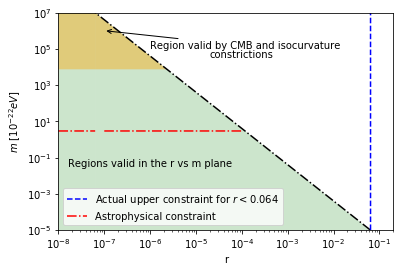
\includegraphics[width=8cm]{SFDMconstraints.png}
\caption{Isocurvature constraints for the SFDM candidate.}\label{constraintsSFDM}
\end{figure}

\textit{Massive complex SFDM model.-} A massive complex scalar field is described by the potential
\begin{equation}
V(|\psi|^2)= m^2|\psi|^2
\end{equation}
As we have shown in appendix [B] when we consider a complex scalar field its dynamics is modified only by the centrifugal term (see eq. \eqref{KGe3}). However as it was demostrated in [referencias] such term does not affect the dynamics of the field at cosmological level, obtaining then that a complex scalar field and a real scalar field have the same cosmological history in the Universe. In this way if we consider that our complex SFDM fulfilled slow-roll conditions during inflation its constrictions for isocurvature perturbations must be the same than in the real field analogue. 


\textit{Self-interacting SFDM scenario with a positive interaction.-} When the massive SFDM scenario is compared with observations there are several discrepancies about the constrictions for the mass of the model. For example (\textcolor{red}{Hablar sobre las constricciones. Que unos ponen como cota inferior la masa de $10^{-21}$ mientras que otros ponen otras cotas que quedarían fuera de las totas de otros experimentos.}). For this reason it is convenient to extend the model and introduce a self-interacting term that can help us to relax this discrepancies. For simplicity we continue considering that the SF does not interact with the inflaton in such case the total potential of the system can be given by
\begin{equation}
V(\phi,|\psi|^2)=V(\phi)+m^2|\psi|^2+\frac{1}{2}\lambda|\psi|^4
\end{equation}
As we have shown in appendix [B] we have 2 different scenarios in this model: a weak interacting and a strong interacting scenario. In the weak interacting model our SFDM behaves effectively as a massive field without auto-interaction, in such case the constrictions obtained by the massive field applies to this scenario. In the other side when the auto-interacting term is big enough we obtain that in the cosmological history of the scalar field we will have a new period where the SFDM behaves as a radiation-like fluid. In this way the constrictions that we have done before will not apply to this model anymore.

Before to start to study the strong scenario notice that we can give general constrictions for the auto-interacting term in terms of the ones that we have made until now. As we can see in appendix [B] we have the weakly self-interacting regime when $m^2\gg \lambda|\psi_i|^2/2$. In fact, thanks to the decreasing behavior of bout scenarios we can consider that this regime is fulfilled always that $m^2\geq \lambda|\psi_i|^2/2$ or equivalently when $\lambda\leq 2m^2/|\psi_i|^2$. If we consider that the SFDM oscillations start at the same moment that the only massive case (which is not really true but we can consider it as a good approximation), using eq. \eqref{phi_im2} we observe that this constriction can be given only in terms of the mass $m$ of the SF as
\begin{equation}
\left(\frac{\lambda}{10^{-96}}\right)\leq 1.2\left(\frac{m}{10^{-22}eV}\right)^{5/2}
\end{equation}
We plot in figure \ref{weakregime} the weak limit obtained by our approximation. However this limit overestimate the value that $\lambda$ since when in the above expression we have an equality the field is not behaved as a dust-like field at all, this behavior is obtained when the $\lambda$ term is completely negligible.
\begin{figure}\label{weakregime}
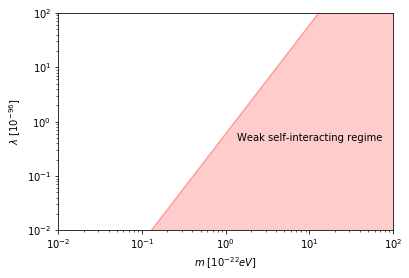
\includegraphics[width=8cm]{weakregime.png}
\caption{Weakly self-interacting regime}
\end{figure} 

In the strong self-interacting regime the SFDM follows an attractor solution \eqref{atractor} during inflation (see appendix [\textcolor{red}{n}]). Then the value that the homogeneous field can have after inflation depends on if $\eta_{att}<\sqrt{2}m/\sqrt{\lambda}\equiv \eta_t$ or not. When $\eta_{att}<\eta_t$ the field follows the attractor solution until $\eta\simeq \eta_t$. Then the scalar field is frozen at that value and starts to oscillate as a massive field when $m\sim H$. 

Notice that we can do two kind of constrictions of our free parameters. Frist, from equation \eqref{initial_c} and taking $|\psi_i|=\eta_t$ we have
\begin{equation}
r<1.2\times 10^{-4}\left[\frac{\left(\frac{m}{10^{-22}eV}\right)^2}{\frac{\lambda}{10^{-96}}}\right]
\end{equation}
While in the other side given the fact that when the SFDM starts its oscillations it behaves as a massive field, the constrictions obtained in the non-interacting field must be fulfilled as well. Matching $\eta_t$ with \eqref{phi_im2} and considering the constriction given in primordial tensor perturbations by eq. \eqref{constm} we obtain
\begin{equation}
\left(\frac{\lambda}{10^{-96}}\right)\leq 1.2\left(\frac{2\times 10^{-4}}{r}\right)^5
\end{equation}
In figure \ref{constraintsSFDMl} we have plotted the above condition that is valid in the weak interacting regime.

\begin{figure}[h]
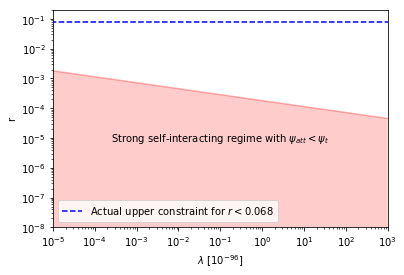
\includegraphics[width=8cm]{lambdavsr.png}
\caption{Isocurvature constraints for the weakly auto-interacting term.}\label{constraintsSFDMl}
\end{figure} 

When $\eta_{att}>\eta_t$ we have that the field follows the attractor solution during all inflation. In this way the initial condition that the SFDM has is given by \eqref{atractor2}
\begin{equation}\label{atractor3}
\eta_{att}^i = \left(2\lambda\int_{\phi_{end}}^{\phi_0}V^{-1}_{,\phi}d\phi\right)^{-1/2}
\end{equation}
Then the SFDM remains frozen at value $\eta_{att}^i$ until $M\sim H$ and then it start to oscillate with a quartic potential. In this scenario the SF density behaves as $\rho_{SFDM}\propto |\psi|^4$ and then we can write $P_{SFDM}=4\delta\psi/\psi_i$. In this way the primordial isocurvature perturbations for a strong-interacting SFDM is given by
\begin{equation}
P_{SFDM}(k)=\left|\frac{2H_*}{\pi\psi_i}\right|^2
\end{equation}
In appendix [N] we show how the initial condition can be related with the value that we see now. Using eqs. \eqref{inilamb2} and \eqref{phi_im2} from appendixes [N], using $g_{*osc}=3.36$ and $g_{s*osc}=3.91$  and considering constrictions [eq] we obtain now
\begin{equation}
r<\frac{1.172\times 10^{-4}}{7^{1/3}f^2(\sigma)}\left[\frac{2\left(\frac{m}{10^{-22}eV}\right)^{3/2}}{\left(\frac{\lambda}{10^{-96}}\right)}\right]^{1/2}
\end{equation}
We show in figure \ref{constraintsSFDMls} constraints given for the strong scenario in terms of tensor-to-scalar ratio. It is necessary to mention that there are some region of parameters where the strong and the weakly scenarios are overlapped in our approximations. This is because the different simplifications that we had consider for our analysis. However this descriptions can give us general considerations for our SFDM models. For example, as we can see in the figure as long as the mass parameter $m$ of the SF decreases, the auto-interacting term must to decrease as well in order to avoid an overproduction of gravitational waves. Comparing figures \ref{constraintsSFDM} and \ref{constraintsSFDMls} we can also notice that when we are in the strong self-interacting regime isocurvature constrictions are more restrictive, since in this scenario the non-detection of gravitational waves could ruled-out SFDM candidates with the most light masses.
\begin{figure}
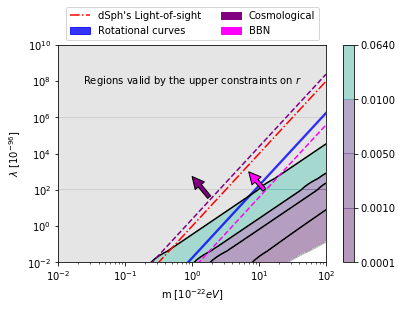
\includegraphics[width=8cm]{stronglamb.png}
\caption{Isocurvature constraints for the strong auto-interacting scenario.}\label{constraintsSFDMls}
\end{figure} 

It is also necessary to be careful that the SFDM does not come to dominate the inflationary process.  This is guarantee by demanding
\begin{equation}
\lambda < \frac{H_*^2 M_p^2}{|\psi_i|^4}
\end{equation}
\textcolor{red}{(Ponerlo en t\'erminos de $r$ y mostrar que se cumple f\'acilmente.)}
\\

Additionally we can see that we can do general constrictions in the potential of the inflaton considering equation \eqref{atractor3}. Notice that this scenario is fulfilled always that
\begin{equation}
\left(\int_{\phi_{end}}^{\phi_0}V_{,\phi}^{-1}d\phi\right)^{-1/2}>2m
\end{equation}
If this scenario is fulfilled we need to avoid isocurvature perturbations, which implies from \eqref{initial_c} that
\begin{equation}
r<\frac{0.6}{\left(\frac{\lambda}{10^{-96}}\right)}\left(\frac{10^{40}}{\int_{\phi_{end}}^{\phi_0}V_{,\phi}^{-1}d\phi}\right)
\end{equation}
where we have taken $10^{-96}$ as natural order of magnitud of the self-interacting regime, which correspond with an ultra-light SFDM. This implies that the natural oder of magnitud of the integral term should be $10^40$. This results can be interpreted as follows: if we consider a self-interacting SFDM candidate that coexist with the inflaton, in order to obtain the strong scenario it is necessary that the above conditions fulfilled. For an ultra-light SFDM this implies that the integral term of the potential should be very large $\sim 10^{40}$. In the other side, if we start in the strong self-interacting regime and for an ultra-light SFDM, in order to obtain the other scenario, $\eta_{att}<\eta_t$, the integral term of the inflaton must be very small. If we can not fulfilled bout conditions this implies that need to be in the weakly self-interacting regime and then it is not possible to obtain a radiation-like period of the SFDM during its cosmological evolution.
\\

\textit{Self-interacting SFDM scenario with a negative interaction.-}
\\
\textcolor{red}{Me faltar\'ia agregar esto, que seg\'un veo es b\'asicamente lo mismo que el caso anterior, pero con una condici\'on extra de que posterior a inflaci\'on no se restaure la simetr\'ia del potencial por oscilaciones resonantes (potencial tipo sombrero mexicano) y por ende de cabida a formaci\'on de cuerdas c\'osmicas. No lo he agregado porque s\'olo he revisado como 3 art\'iculos y quer\'ia estar bien seguro que todas estas cosas tambi\'en aplican a un campo escalar ultra-ligero.}

\textit{What about a coupling term between the inflaton and the SFDM?}
\\

\textcolor{red}{Tambi\'en pensaba agregar esta secci\'on. Seg\'un he visto lo que hace el acomplamiento es justificar el valor grande de la condici\'on inicial del campo homogeneo (ya que el m\'inimo se ve cambiado por el acoplamiento con el inflat\'on). Sin embargo, tengo entendido que hay un poco m\'as de problemas cuando hay un potencial cu\'artico. El estudio completo se hace en este paper: https://arxiv.org/pdf/1507.00119.pdf }

\subsection{Curvaton scenario}

In the curvaton scenario it is assumed that during inflation there was an extra scalar field that coexist with the inflaton and its classical dynamics was negligible (its energy density was sub-dominant during inflation). Then, similar to the SFDM scenario, this scalar field obtained quantum fluctuations, leading to the generation of primordial isocurvature perturbations. If the curvaton field is long lived (at least its life must be longer than the inflaton one) it starts to oscillate when the Hubble scale $H$ approaches the curvaton mass (see appendix [B]) shortly before or after the inflaton decays to radiation. During its oscillation phase, this curvaton field starts to behave as dust and then its perturbations are reduced slower than the ones associated with the inflaton [ref]. If the curvaton decays to radiation when its quantum fluctuations dominates over the inflaton ones, we can obtain a scenario where curvaton quantum fluctuations can dominate the early Universe and give place to be the totality of the initial adiabatic perturbations (ref). In our formalism, such scenario is obtained when $T_{RS}>>1$ or equivalently when we consider in our analysis $\sin\Delta = 0$ (ref), in such case we obtain that the tensor-to-scalar ratio in the pure curvaton scenario is $r=0$. 

In the last few years people has started to study curvaton models but considering that the curvaton field does not constribute for the totality of the primordial adiabatic perturbations, instead, it contributes to a fraction of the total curvature perturbations, while the remaining one was produced by the inflaton (ref). Notice that such scenario is obtained if $0<\cos\Delta <1$. It is also usual to redefine a new parameter in this model $R= [\cot^2\Delta]_{k_0}$ which can be related with the curvaton-to-inflaton density fraction of primordial curvature perturbations. Then, the primordial adiabatic perturbations can be written from \eqref{PrAs} as
\begin{equation}\label{PCr}
\mathcal{P}_R(k)=A_r\left(\left(\frac{k}{k_{0}}\right)^{n_s^\phi-1}+R\left(\frac{k}{k_{0}}\right)^{n_s^\psi-1}\right)
\end{equation}
where $n_s^\phi-1 = -6\epsilon_\phi+2\eta_{\phi\phi}$ and $n_s^\psi-1 = -2\epsilon_\psi+2\eta_{\psi\psi}$.
The total spectral index ($n_s-1=d\ln P_R/d\ln k$) is given then by
\begin{equation}
n_s-1=\frac{n_s^\phi+R n_s^\psi}{1+R}-1
\end{equation}

An advantage of this kind of models is that it can help to single inflationary models that at the moment could be considered as ruled-out by the data (but that could be well motivated theoretically) to remain in the competition in the inflationary zoo. As an example in (referencia de Curvaton after Planck) it was studied in a Bayesian framework several inflationary models with an extra light scalar field with a quadratic-like potential \textcolor{red}{(Checar bien esta parte)}. In such study it was obtained that one of the most preferable scenarios is a quartic-like inflationary potential with our extra scalar spectator. However it is necessary to notice that such scenario is favorable only in the limit where the curvaton produced nearly the totality of the primordial adiabatic perturbations, i.e. when $R>>1$. If in the other side we allow that our parameter $R$ takes whichever value, we could expect that more chaotic-like inflationary potentials could continue fitting observations. In fact when we consider the chaotic potential $V(\phi)=(1/2)m_p\phi^p$ for the inflaton and the  potential $V(\psi)= (1/2)M^2\psi^2$ for the curvaton, the spectral index $n_s$ is rewritten as
\begin{equation}
\label{nsexplicit}
n_s-1\approx -\frac{1}{1+R}\frac{2(2+p)}{4N+p}+\frac{R}{1+R}\left[-\frac{2p}{4N+p}+\frac{2M^2}{3H_*^2}\right]
\end{equation}
where  $N$ is the number of e-folds produced before our scales left the horizon and it is usually used $N=50\sim 60$. In the above equation we have used the Friedman equation in the slow-roll approximation for the term containing $M$. In this way from \eqref{Tensortoscalar} the tensor to scalar ratio in this model is given by
\begin{equation}\label{tensortoscalar}
r=\frac{16\epsilon_\phi}{1+R}
\end{equation}		
If we use \eqref{tensortoscalar} into \eqref{nsexplicit} we have 
\begin{equation}
n_s-1=-\frac{(2+p)}{8p}r+\left[1-\frac{(4N+p)}{16p}r\right]\left[\frac{2}{3}\frac{M^2}{H^2}-\frac{2p}{4N+p}\right]
\end{equation}
where we have obtained a relation between the spectral index and the tensor-to-scalar ratio which are well constrain by the data. Notice that in the limit when the curvaton dominates completely the adiabatic perturbations ($r\simeq 0$) and considering the mass of the curvaton negligible compared with the Hubble parameter (i.e. $M<<H$) we obtain that $n_s-1\simeq p/(120+p/2)$ and then the observational constrains for the spectral index means that the inflaton field must be close to be a quartic potential, $p=4$. Such result can be observed in figure \ref{nvsr}, where we have plotted the above equation neglecting $M/H$ and letting $R$ to vary using as our only constriction for it the actual upper constraint on $r$. In such figure we can observe an upper an lower value for $n_s$ in terms of $r$ which is obtained when we consider $N=60-50$ e-folds at the moment when our scales left the horizon. In the other side when we allow $M/H$ to vary using as our constriction that $M/H<1$ (in order to obtain quantum fluctuations for the curvaton during inflation) we can obtain that for some regions of parameters more chaotic like potentials can fit well the data. Such results can be observed in figures \ref{curv50} and \ref{curv60} where we have plotted contour plots for $r$ from the above equation in the $M/H$ vs $n_s$ plane. In this way we have seen the big advantage of adding this new degree of freedom to a simple chaotic-like model of inflation.
\begin{figure}
\centering
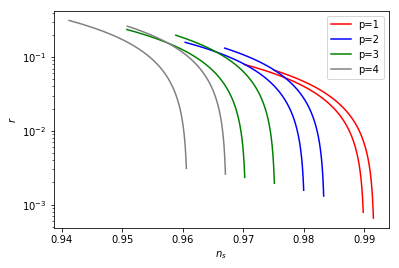
\includegraphics[width=0.4\textwidth]{nvsr}
\caption{Possible values in the n vs r plane when we allow $R$ to vary. The values that can be produced by the models are the ones between the two limits plotted in the figure.\textcolor{red}{(Tratar de pintar las regiones entre las l\'ineas y poner los datos de Planck para que se vea mejor.)}}
\label{nvsr}
\end{figure}
% * <epadilla@fis.cinvestav.mx> 2018-04-29T03:33:02.572Z:
%
% ^.
\newpage
\begin{figure}[h]
\centering
\begin{subfigure}[b]{\textwidth}
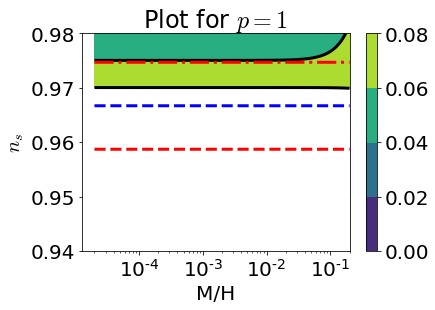
\includegraphics[width=0.4\textwidth]{p150.png}
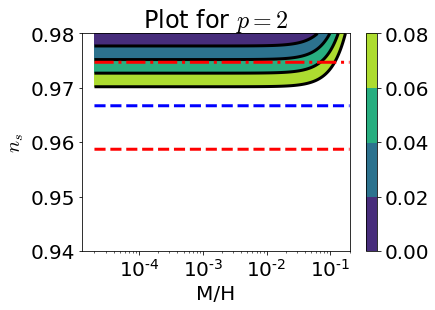
\includegraphics[width=0.4\textwidth]{p250.png}\\
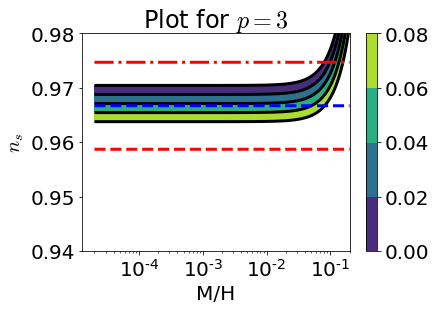
\includegraphics[width=0.4\textwidth]{p350.png}
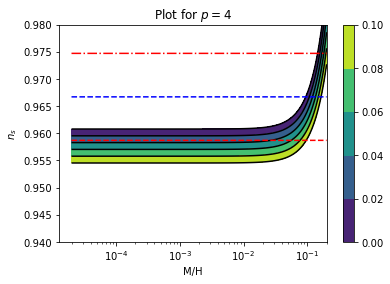
\includegraphics[width=0.4\textwidth]{p450.png}
\label{curv50}
\end{subfigure}
\caption{Inflationary constraints in the $M/H$ vs $n_s$ plane for $N=50$ e-folds. We plotted contour regions for $0<r<0.1$.}
\begin{subfigure}[b]{\textwidth}\centering
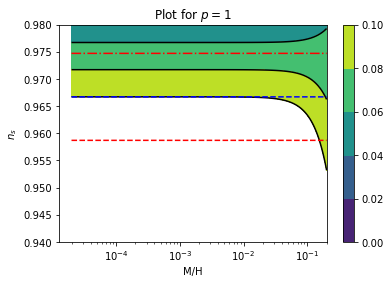
\includegraphics[width=0.4\textwidth]{p160.png}
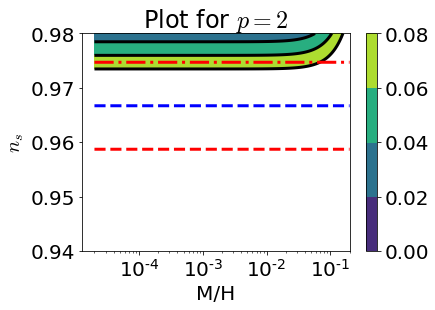
\includegraphics[width=0.4\textwidth]{p260.png}\\ 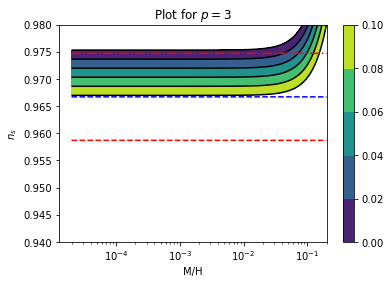
\includegraphics[width=0.4\textwidth]{p360.png}
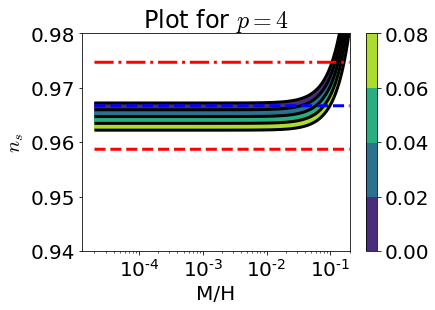
\includegraphics[width=0.4\textwidth]{p460.png}
%\captionof{figure}
%{\footnotesize{A }}
\label{curv60}
\end{subfigure}
\caption{Inflationary constraints in the $M/H$ vs $n_s$ plane for $N=60$ e-folds. We plotted contour regions for $0<r<0.1$.}
\end{figure}
\section{Constraining two field models with last data}
A
\section{Conclusions}
\appendix
\section{Slow-Roll index}

In this appendix we define the slow roll indexes used in our calculation. We have:
\begin{subequations}
\begin{equation}
\epsilon_i = \frac{1}{16 \pi G}\left(\frac{V_i}{V}\right)^2, \ \ \ \ \ \text{where $i=\phi,\psi$}
\end{equation}
\begin{equation}
\eta_{ij}=\frac{1}{8\pi G}\left(\frac{V_{ij}}{V}\right)
\end{equation}
\end{subequations}
where $V_i = \partial V/\partial \phi_i$. In the other side we have
\begin{equation}
\epsilon \equiv \frac{1}{16\pi G}\left(\frac{V_\sigma}{V}\right)^2\simeq \epsilon_\phi+\epsilon_\psi
\end{equation}
and
\begin{eqnarray}
\eta_{\sigma\sigma}&=&\eta_{\phi\phi}\cos^2\theta + 2\eta_{\phi\psi}\cos\theta\sin\theta+\eta_{\psi\psi}\sin^2\theta\nonumber \\
\eta_{\sigma s}&=&(\eta_{\psi\psi}-\eta_{\phi\phi})\sin\theta\cos\theta + \eta_{\phi\psi}(\cos^2\theta-\sin^2\theta)\\
\eta_{ss}&=&\eta_{\phi\phi}\sin^2\theta - 2\eta_{\phi\psi}\cos\theta\sin\theta+\eta_{\psi\psi}\cos^2\theta\nonumber 
\end{eqnarray}
\section{Generalities for SFDM models}

In order to constraint our SFDM model using our isocurvature constrictions it is necessary to relate the value of the field now with the value that it has during inflation. This constrictions depend on the SFDM model that we consider. In this appendix we analyze the evolution of different models for SFDM and then in [section], with the help of isocurvature constrictions, try to constraint the free parameters of our models. 

In this scenario our scalar field can be coupled or not with the inflaton, then we consider the general potential of the form $V(\phi,|\psi|^2)$, where in such case it is convenient to work using a Madelung transformation [ref]
\begin{equation}
\psi = \eta \exp[i\theta]
\end{equation}
where $\eta\equiv |\psi|$ is the magnitude of field $\psi$ and $\theta$ its phase. Notice that in order to obtain a slow-roll approximation it is neccesary that $|\theta|<<1$ and $\eta$ fulfill the slow-roll condition during inflation. Since we are interested in the complete history of the SFDM in the Universe let us rewrite and separate the KG equation in its real and imaginary components as
\begin{subequations}\label{KESFDM}
\begin{equation}\label{KGe1}
\ddot\eta+3H\dot\eta+\frac{dV}{d|\psi|^2}\eta-\omega^2\eta= 0,
\end{equation}
\begin{equation}\label{KGe2}
\dot\omega \eta + (2\dot\eta+3H\eta)\omega=0
\end{equation}
\end{subequations}
where $\omega = \dot \theta$, while the equation of the inflaton field continue being eq. \eqref{KGEq}. Equation \eqref{KGe2} can be exactly integrated as
\begin{equation}
\frac{d}{dt}\left(a^3\eta^2\omega\right)=0
\end{equation}
wich implies that 
\begin{equation}
a^3\eta^2\omega=Q
\end{equation}
where $Q$ is a charge of the SF \textcolor{red}{(poner referencia Abril y las que hay dentro)}. Using this last equation in \eqref{KGe1} we obtain finally
that the radial component of the scalar field fulfill
\begin{equation}\label{KGe3}
\ddot\eta+3H\dot\eta+M^2\eta-\frac{Q^2}{\eta^3}= 0,
\end{equation}
The term containing $Q$ is obtained by the complex nature of the SF [ref] an it can be interpreted as a "cenrifugal force" [ref]. In the other side $M\equiv dV/d|\psi|^2$ can be interpreted as an effective mass term of the scalar field. Notice here that if we consider $Q^2/\eta^3\ll 1$ and we suppose that the SFDM candidate fulfill the slow-roll condition during inflation, the field $\eta$ will remain frozen at value $\eta_i$ until $H\sim M$. Then, when $H\sim M$ it will start to evolve depending on the behavior of the effective mass term.
\begin{center}
\textit{A real massive SFDM candidate}
\end{center}

A massive real scalar field is described by the potential 
\begin{equation}
V = \frac{1}{2}m^2\psi^2
\end{equation}
Then we have that in equations \eqref{KESFDM} $\eta=\psi$ and $\theta=0$ which implies that $\omega=0$ and then $Q = 0$. We consider for simplicity that our SFDM candidate was not coupled with our inflaton field, in such case we can rewrite the total potential during inflation as

\begin{equation}
V(\phi,|\psi|)=V(\phi)+\frac{1}{2}m^2\psi^2
\end{equation}
In this way we can see that $M^2=m^2$. As we mentioned above when $H\gg m^2$ the therm that contains $m^2$ in equation \eqref{KGe1} can be neglected and then the field $\psi$ remains frozen at its initial value by Hubble dragging during the early universe. Then, when $m\sim H$ the SFDM starts to evolve. Given that the effective mass of the field is constant, the dependence of phi respect to $a$ during the oscillating phase is $\psi\sim 1/a^{3/2}$, while its density behaves as $\rho_{\psi}\sim 1/a^3$  [ref]. In this way we can write the scalar density of our field as
\begin{equation}\label{rhosfdm}
\rho_\psi = \left\lbrace\begin{array}{ll}
\frac{1}{2}m^2\psi_i^2 & \text{where }H\gg m \\
\frac{1}{2}m^2\psi_i^2\left(\frac{a_{osc}}{a}\right)^3 & \text{where }H\ll m
\end{array}\right .
\end{equation}

The typical mass that it is considered for a SFDM candidate is around $10^{-22} eV$ [ref] which implies that the field should starts its oscilations during a radiation-dominated Universe [ref]. During this period the Hubble parameter evolves in terms of the scale factor as $H\propto a^{-2}$. We can solve the KG equation \eqref{KGEq} exactly during this period in terms of the scale factor obtaining
\begin{equation}
\psi = \psi_i\Gamma\left(\frac{5}{4}\right)\left(\frac{4H}{m}\right)^{1/4}J_{1/4}\left(\frac{m}{2H}\right)
\end{equation}
where $\psi_i$ is the scalar field value during inflation and it was imposed initial condition for $\psi$ in such a way that when $m/H\rightarrow 0$ we obtain $\psi\rightarrow\psi_i$. If now we consider that in the above expression we obtain the $H\ll m$ behavior of equation \eqref{rhosfdm} when $m/H\rightarrow \infty$ we obtain that
\begin{equation}\label{m_osc}
\frac{m^2}{H_{osc}^2}\simeq 2.68
\end{equation}
whit $H_{osc}$ the value of the Hubble parameter at the momment when the SFDM starts its oscilations.

Using the relation for a radiation-dominated Universe
\begin{equation}
\rho_r = 3M_p^2H^2=\frac{\pi^2}{30}g_*T^4
\end{equation}
where $M_p\equiv (8\pi G)^{-1/2}$ is the Planck mass and $g_*$ the effective degrees of freedom, and \eqref{m_osc} we can obtain the temperature when our SFDM particle starts its oscilations
\begin{equation}
T_{osc}\simeq 0.5 keV\left(\frac{g_{*osc}}{3.36}\right)^{-1/4}\left(\frac{m}{10^{-22}eV}\right)^{1/2}
\end{equation}
where we have left the values inside the parentesis for $g_{*osc}$ and $m$ by convenience since our ultra-light particle starts its oscilations during a radiation-dominated era. 

Finally, using that the entropy of the Universe is conserved we can express the actual density of SFDM particles as
\begin{equation}
\rho_{DFDM0}=\frac{1}{2}m^2\psi_i^2\frac{s_0}{s_{osc}}
\end{equation}
where the subscript ``$0$" indicates quantites at present. Using the relation that $s=\frac{2\pi}{45}g_{*}T^3$ and the constraints given by Planck [ref] for the actual amount of Dark Matter content $\Omega_{DM}h^2=0.1186\pm 0.0020$ $68\% C.L., TT. + lowP+\text{lensing}$ we finally obtain 
\begin{equation}\label{phi_im2}
|\psi_i|^2\simeq\frac{10^{34}GeV^2}{0.6}\left(\frac{g_{*osc}}{3.36}\right)^{-3/4}\left(\frac{g_{s*osc}}{3.91}\right)\left(\frac{m}{10^{-22}eV}\right)^{-1/2}
\end{equation}

\begin{center}
\textit{A complex massive SFDM candidate}
\end{center}

Let us consider now a complex scalar field which is not coupled with the inflaton. This scenario is obtained by considering a complete potential of the form
\begin{equation}
V(\phi,|\psi|^2)=V(\phi)+m^2|\psi|^2
\end{equation}
As we saw in the real case in order to avoid isocurvature perturbations it is neccesary that the scalar field starts from a high value of $\eta_i$ in such case we can ignore the last term in eq. \eqref{KGe3}. In the other side considering the same argument than in the real case we can see that the SF value remains frozen until $m\sim H$ and then it starts to oscilate. In [ref] it was demostrated that a massive complex scalar field behaves equivalent to the real case at cosmological levels, being such term important only at galactic levels. Taking this in mind we can consider that all what we did in the real case applies to this case and then a complex scalar field has the same constrictions than the real one. 
\begin{center}
\textit{Self-interacting Scalar Field with a positive interaction}
\end{center}

We consider in this section a self-interacting scalar field with a positive interaction. This scenario is described by the potential associated with the SFDM
\begin{equation}
V = m^2|\psi|^2+\frac{1}{2}\lambda |\psi|^4
\end{equation}
If we consider that our SF was not coupled with the inflaton we will have that the complete dynamics of the system is obtained with the full potential 
\begin{equation}
V(\phi,|\psi|^2)=V(\phi)+m^2|\psi|^2+\frac{1}{2}\lambda|\psi|^4
\end{equation}
Notice that the effective mass of the field is $M^2=m^2+\lambda|\psi|^2$. Thanks to the slow-roll condition imposed during inflation the effective mass of the field remains constant at $M^2=m^2+\lambda|\psi_i|^2$ until $M\sim H$, then, depending on what term dominates in $M^2$ we can have two different kind of dynamics. 
\\

\textit{Weakly self-interacting regime.-} This limit is obtained when the constant term in $M^2$ dominates, it is when
\begin{equation}\label{consw}
m^2\gg \frac{1}{2}\lambda|\psi_i|^2
\end{equation}
In this regime it is possible to ignore the autointeracting term in equation \eqref{KGe3} when oscilations of the scalar field begins. However, because when we ignore such term the field behaves as a massive field and as we can see in \eqref{rhosfdm} the field value always decreases, the autointeracting term never dominates and then all the cosmological history of the SFDM candidate is the same than in the pure massive scenario. 
\\

\textit{Strong self-interacting regime.-} This scenario is obtained when 
\begin{equation}
m^2\ll \frac{1}{2}\lambda|\psi_i|^2
\end{equation}
If the above expression is fulfilled we can see that at the moment when the SFDM starts its oscillations ($M\sim H$) its effetive mass is quadratic in the field. In that regime the scalar field evolves as $\psi\sim 1/a$ and its energy density as $\rho_{\psi}\sim 1/a^4$ behaving as radiation. Then, when $m^2 \sim \frac{1}{2}\lambda|\psi_t|^2$ we obtain that the effective scalar field mass is now constant, obtaining the dust-like behavior that we analyze before. Here $\psi_t$ is the valur of the SF at the momment when the constant term in $M$ starts to dominate. In this way we can write the history of the scalar density of our field as
\begin{equation}\label{rhosfdmlam}
\rho_\psi = \left\lbrace\begin{array}{ll}
\frac{1}{2}\lambda^2|\psi_i|^4 & \text{where }H\gg \lambda|\psi_i|^4 \\
\frac{1}{2}\lambda|\psi_i|^4\left(\frac{a_{osc}}{a}\right)^4 & \text{where }H_t\leq \lambda|\psi_i|^4\leq H\\
m^2|\psi_t|^2\left(\frac{a_t}{a}\right)^3 & \text{where } m^2\leq H_t
\end{array}\right .
\end{equation}
Here sub-index $t$ means quantities measured at transition between radiation and dust behavior of the SFDM and
\begin{equation}\label{inilamb}
|\psi_i|^2=\left[\frac{2m^2}{\lambda}|\psi_t|^2\right]^{1/2}\left(\frac{a_t}{a_{osc}}\right)^2
\end{equation}
Notice that we have consider for simplicity a direct transition between radiation-like to dust-like densities. 

In order to continue it is necessary to specify the value of $a_t$ and $a_s$. Since the auto-interacting KG equation can not be solved exactly it is necessary to work with approximated solutions. In [Suarez and Chavanis] it was obtained using a pure approximated description of the system the relation (see its equation 80 and 86)
\begin{subequations}
\begin{equation}\label{atoveras}
\left(\frac{a_t}{a_{osc}}\right)^2=\frac{3}{7^{1/3}f^2(\frac{a_s}{r_S})}
\end{equation}
where 
\begin{equation}
f(\sigma)=\frac{1}{s^{1/3}(1+4s)^{1/6}}
\end{equation}
with
\begin{equation}
s=\frac{4\sigma-1+\sqrt{(4\sigma-1)^2+12\sigma}}{6}
\end{equation}
\end{subequations}
Additionally $r_S=2mG/c^2$ and $a_s=\hbar^2\lambda/4\pi m$ which implies that $a_s/r_s=\lambda M_p^2/m^2$, where $M_p^2\equiv\hbar c/8\pi G$ is the Planck mass. Rearranging it in a more convenient way we have
\begin{equation}
\sigma \simeq 5.93\times 10^{
2}\left(\frac{m}{10^{-22}eV}\right)^{-2}\left(\frac{\lambda}{10^{-96}}\right)
\end{equation}
Notice that when $a_t/a_{osc}\simeq 1$ i.e. when $3/(7^{1/3}f^2(\sigma))\sim 1$ there is not a radiation-like epoch. This scenario should match with the non-interacting scenario that we studied before.

Inserting equation \eqref{atoveras} into \eqref{inilamb} follows
\begin{equation}\label{inilamb2}
|\psi_i|^2=\frac{3}{7^{1/3}f^2(\sigma)}\left[\frac{2m^2}{\lambda}|\psi_t|^2\right]^{1/2}
\end{equation}
But the above relation means that it is enough to match the value of the field at $\psi_t$ with the value at present and then with the above relation we can obtain the value that the SF had during inflation. In the other side notice that at $a_t$ the scalar field starts to behave as dust with an effective mass $M^2=m^2+\lambda|\psi_t|^2$. This implies that dust-like oscillations of the SF start a little before than the non-interacting case. If we allow $m$ to be ultralight $(m\sim 10^{-22}eV)$ and thanks to the fact that $m^2$ is of the same order that $\lambda|\psi_t|^2$ we can see that such oscillation starts at the same epoch that the non-interacting case does. In fact we can see that because the decreasing behavior of the SF at that period ($\psi\sim 1/a^{3/2}$) the auto-interacting term left to be important quickly and then the dynamics of the field is quickly described only by the mass term $m$. We consider. for simplicity that once the dust-like behavior starts, the dynamics is described similar to  the non-interacting case, in such case the condition \eqref{phi_im2} is fulfilled by our SF as well, but interchanging subindex $i$ with $t$\footnote{In fact this is a lower boundary for the strong auto-interacting case.}.
\\

\textit{Attractor behavior of the SF during inflation.-} In the strong self-interacting regime the SFDM follows the attractor solution [https://arxiv.org/pdf/1211.3535.pdf]
\begin{equation}\label{atractor}
\eta_{att} =\left(2\lambda\int_{\phi}^{\phi_0}V^{-1}_{,\phi}d\phi\right)^{-1}
\end{equation}
where $\phi_0$ is the value of the inflaton at the beggining of inflation (when remains $\sim \ 60$ e-folds for the end of inflation). We can identify two possible scenarios in the above equation:
\begin{itemize}
\item $\eta_{att}>\sqrt{2}m/\sqrt{\lambda}$

In this scenario the dynamics of the inflaton is given by \eqref{atractor} during inflation which implies that the initial condition of the field after inflation is given by
\begin{equation}\label{atractor2}
\eta_{att}^i = \left(2\lambda\int_{\phi_{end}}^{\phi_0}V^{-1}_{,\phi}d\phi\right)^{-1/2}
\end{equation}
where $\phi_{end}$ is the value of the inflaton at the end of inflation. We need to specify that it is the value of the field in the early Universe until its oscilations starts (i.e. $M\sim H$). This initial condition can be compared with \eqref{inilamb2} obtaining then
\begin{equation}\label{inilamb2}
\left(2\int_{\phi_{end}}^{\phi_0}V^{-1}_{,\phi}d\phi\right)^{-1}=\frac{3}{7^{1/3}f^2(\sigma)}\left(2m^2\lambda|\psi_t|^2\right)^{1/2}
\end{equation}


\item $\eta_{att}<\sqrt{2}m/\sqrt{\lambda}$

In this scenario the SFDM follows the attractor solution until $\eta\simeq \sqrt{2}m/\sqrt{\lambda}$. Then the SF reaches $\eta_i=\sqrt{2}m/\sqrt{\lambda}$ for the rest of inflation. Notice that this value correspond with the upper value that the weakly self-interacting regime allows. Then the field starts to evolve when $H\sim M$ behaving as a massive SF. In this way, for this scenario, the constrictions given in the non-interacting case apply but where the initial condition are also fixed by $\eta_i$. Using both relations we can obtain the value that $\lambda$ should have, which is
\begin{equation}
a\end{equation}
\end{itemize}

\section{Papers} 
Aqu\'i pondré de mientras los links de los papers que he revisado:

https://arxiv.org/pdf/1211.3535.pdf

https://arxiv.org/pdf/1712.05364.pdf

https://arxiv.org/pdf/1505.00639.pdf

https://arxiv.org/pdf/astro-ph/0306500.pdf

https://arxiv.org/pdf/1708.05681.pdf

https://arxiv.org/pdf/1211.3535.pdf

https://arxiv.org/pdf/1507.00119.pdf

https://arxiv.org/pdf/1801.07409.pdf

https://arxiv.org/pdf/1305.5338.pdf
\end{document}

